% !TEX root = ../../numb3rs.tex
\newpage
\subsection{304: The Mole\label{304}}

In this episode, Charlie and the FBI team try to find a mole in the federal government that is leaking secrets to the Chinese.

\temph{Face Recognition}

In this episode, Charlie uses a face recognition program to identify the people that appear in a surveillance video. He uses a technique called \emph{Eigenfaces} to do this. Before understanding how this technique works, we have to introduce a statistical technique called \emph{Principal Component Analysis}.

%%%%%%%%%%
\noindent \textbf{\large Principal Component Analysis} \\
%%%%%%%%%%

Principal Component Analysis or PCA is used to reduce the \emph{dimensionality} of a set of data. We will motivate PCA with a simple example. Suppose that as a curious young scientist, you are interested in the properties of apples. You go to the supermarket, buy 8 different apples, and then return home and measure the volume and mass of each apple. Your results might look like this:

	\begin{figure}[H]
	\centering
	\begin{tabular}{ccc}
	Apple \# & Mass & Volume \\
	1 & 0.15 & 10.5 \\
	2 & 0.05 & 2.5 \\
	3 & 0.18 & 8.5 \\
	4 & 0.10 & 5.5 \\
	5 & 0.25 & 13.5 \\
	6 & 0.35 & 19.5 \\
	7 & 0.40 & 15.5 \\
	8 & 0.22 & 11.5 
	\end{tabular}
	\end{figure}

It is hard to notice any pattern in the data just by looking at the table. However when the data is plotted on graph paper, it becomes clear that the two measurements are related. In fact, they almost lie along a straight line:
	\begin{figure}[H]
	   \centering
	   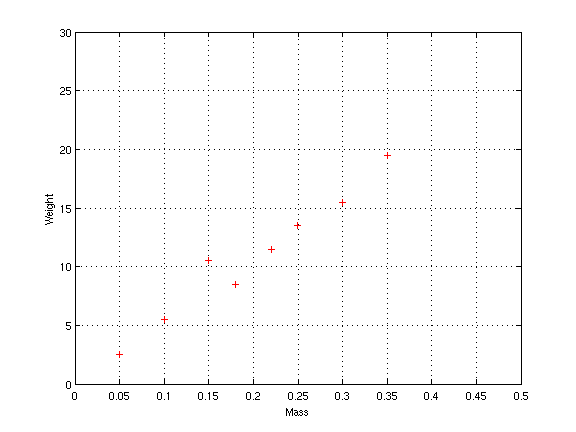
\includegraphics[width=0.6\textwidth]{season3/304/images/applegraph1.png} 
	\end{figure}

Finding the pattern by drawing a graph worked because there were only 2 measurements per apple, and so the result was a 2 dimensional graph. But what if instead we measured 10 features per apple? Then we would need to draw a 10-dimensional graph to look for patterns. That is clearly impossible -- when was the last time you found 10 dimensional graph paper??!! \\

	\begin{enumerate}[1.]
	\item Create a matrix $X$ that contains all of the measurements. Each row of the matrix corresponds 	to a single observation and each column corresponds to a measurement.
	\item Compute the \emph{mean training vector} by averaging together all of the rows of $X$. Call the mean vector $u$.
	\item Subtract u from every row of matrix $X$, to produce a new matrix $Y$.
	\item Compute the \emph{covariance matrix} $C$ of $Y$, using the following formula:
		\[
		C=Y^T Y
		\]
	\item Now we solve the following equation:
		\[
		C \vec{x} = \lambda \vec{x}
		\]
	where $x$ is a vector and is a number. In general there are many values of $x$ and that make this equation true. The possible values of  are called the \emph{eigenvalues} of $C$, and the corresponding solutions for $x$ are called its \emph{eigenvectors}. \\
	\end{enumerate}

We will illustrate PCA by applying it to our apple example. In Step 1, we create a matrix $X$ storing all of the data. The matrix looks like this: 
	\[
	X= 
	\begin{bmatrix}
	0.15 & 10.5 \\
	0.05 & 2.5 \\
	0.18 & 8.5 \\
	0.10 & 5.5 \\
	0.25 & 13.5 \\
	0.35 & 19.5 \\
	0.30 & 15.5 \\
	0.22 & 11.5 
	\end{bmatrix}
	\]
Then we compute the mean, which is $u = (0.212,10.875)$. The result of Step 3 is a new matrix $Y$ where the mean has been subtracted off of every row of $X$: 
	\[
	Y=
	\begin{bmatrix}
	-0.05 & -0.375 \\
	-0.15 & -8.375 \\
	-0.02 & -2.375 \\
	-0.10 & -5.375 \\
	0.05 & 2.625 \\
	0.15 & 8.265 \\
	0.10 & 4.625 \\
	0.02 & 0.625
	\end{bmatrix}
	\]
Step 4 gives us the following covariance matrix: 
	\[
	C=
	\begin{bmatrix}
	0.0708 & 3.7600 \\
	3.7600 & 207.8750 
	\end{bmatrix}
	\]
Finally, we compute the eigenvalues and eigenvectors. The eigenvalues are about 208 and 0.003, and the eigenvectors are $(0.0181, 0.999)$ and $(-0.999,0. 0181)$. The two eigenvectors give us a new set of coordinates that explain the data more compactly. That is, the results of PCA say that the data lies mostly along the vector $(0.0181, 0.999)$, since the corresponding eigenvalue is so much larger than the other. In fact, if we extend the vector $(0.0181, 0.999)$ and overlay it on the graph of training exemplars, we see that the majority of apples lie along the line:
	\begin{figure}[H]
	   \centering
	   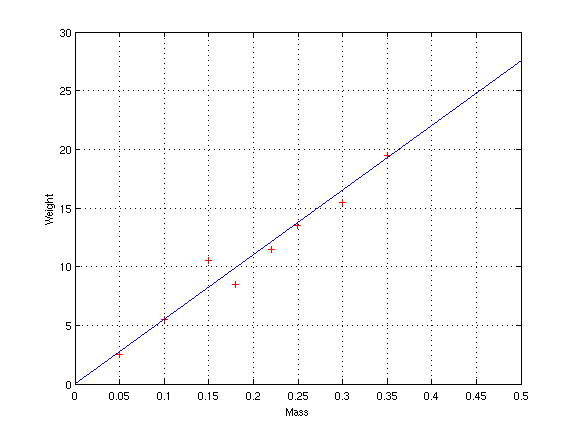
\includegraphics[width=0.6\textwidth]{season3/304/images/applegraph2.png} 
	\end{figure}
In other words, PCA gives us a new coordinate system that allows us to represent the data more compactly instead of using the normal $x$- and $y$- coordinate system. Since most of the apples lie along the line, we can represent each apple with a single number -- its distance from the origin along the line -- instead of the two numbers required by the $x$- and $y$- coordinate system. PCA has given us a way to convert 2-dimensional data to 1 dimension. \\


\noindent\textbf{\large Eigenfaces} \\

Now let us switch from apples to faces. Eigenfaces is a technique that tries to reduce the dimensionality of face data, just like how we reduced the dimensionality of apple data above. \\

To understand how eigenfaces work, we have to understand how images are stored in a computer. A digital image is represented as a set of \emph{pixels} or points of light. For example, each of the face images shown to the right is stored as a $40\times 40$ grid of pixels, and each pixel has a brightness value from 0 to 255. Mathematically, we can think of an image as a vector of length 1600 (since $40\cdot 40=1600$), where each entry in the vector is in the range $[0,255]$. A specific image is represented as a single point in this high dimensional space. \\

How would we go about comparing two face images to decide if they are of the same person? One idea would be to compare the brightness values of the two images pixel-by-pixel and to declare a match if all of the pixel values were similar. We could accomplish this by computing the \emph{Euclidean distance} between the two points in the high dimensional space. Unfortunately, this approach does not work, because two pictures of the same person can be just different enough such that no two pixels actually have the same value. For example, the four images below are of the same person, but the pixel values in every one of them are different. \\
	\begin{figure}[H]
	  \centering
	  \begin{minipage}[b]{0.2\textwidth}
	    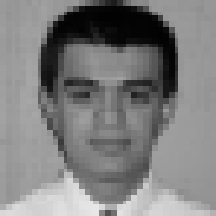
\includegraphics[width=1.08\textwidth]{season3/304/images/face1.jpg}
	  \end{minipage}
	\hspace{0.2cm}
	  \begin{minipage}[b]{0.2\textwidth}
	    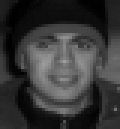
\includegraphics[width=1.01\textwidth]{season3/304/images/face2.jpg}
	  \end{minipage}
	  \hspace{0.2cm}
	  \begin{minipage}[b]{0.2\textwidth}
	    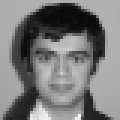
\includegraphics[width=1.08\textwidth]{season3/304/images/face3.jpg}
	  \end{minipage}
	  \hspace{0.2cm}
	   \begin{minipage}[b]{0.2\textwidth}
	    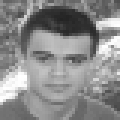
\includegraphics[width=1.08\textwidth]{season3/304/images/face4.jpg}
	  \end{minipage}
	  \end{figure}
In fact, virtually any two images of the same person are going to be at least slightly different and thus be represented as different vectors. It turns out that the number of possible images of the same person is unbelievably large. Suppose we either add or subtract one brightness value from every pixel in one of the above images. This would change the image very slightly but the face would still be recognizable. How many possible ways are there to do this? The answer is $2^{1600}$, or about $10^{480}$. This is an enormously large number; it is many times more than the number of atoms in the universe! \\

Our approach suffers from what is called the \emph{curse of dimensionality}: we are representing our images in a way that is too complicated. Our data has too many degrees of freedom compared to what we need to accurately represent a face. \\

The technique Charlie uses to address this problem is called Eigenfaces. The idea is to transform a face image into a much lower dimensional space that represents only the most important parts of a face. To apply the Eigenface technique, we first collect a \emph{training set} of many (hundreds or thousands) of facial images. Each of the training images is represented as a vector of length 1600, as we saw before. Then we create a matrix $X$ that contains all of the training vectors, one per row. The resulting matrix has size $N\times 1600$, where $N$ is the number of training images. Then we perform PCA on the matrix using the steps given above. Just like before, PCA is used to reduce the dimensionality of the face data. The result is a set of eigenvalues and eigenvectors, as before, but researchers have given eigenvectors of faces a special name: eigenfaces. Usually only a small number (e.g. 10) of eigenfaces are kept after PCA is performed. Each of these eigenfaces is a sort of "prototype" of some general face characteristics. Here are what some Eigenfaces look like: \\
	\begin{figure}[H]
	  \centering
	  \begin{minipage}[b]{0.2\textwidth}
	    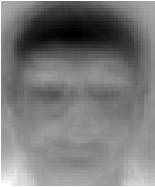
\includegraphics[width=\textwidth]{season3/304/images/eigenface1.jpg}
	  \end{minipage}
	\hspace{0.2cm}
	  \begin{minipage}[b]{0.2\textwidth}
	    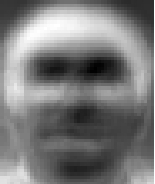
\includegraphics[width=1.01\textwidth]{season3/304/images/eigenface2.jpg}
	  \end{minipage}
	  \hspace{0.2cm}
	  \begin{minipage}[b]{0.2\textwidth}
	    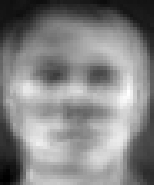
\includegraphics[width=\textwidth]{season3/304/images/eigenface3.jpg}
	  \end{minipage}
	  \hspace{0.2cm}
	   \begin{minipage}[b]{0.2\textwidth}
	    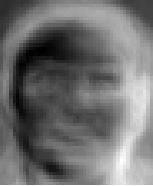
\includegraphics[width=0.98\textwidth]{season3/304/images/eigenface4.jpg}
	  \end{minipage}
	  \end{figure}
Any given face can be encoded as a combination of these eigenfaces. For example, your face might be 10\% of the first eigenface, 30\% of the second eigenface, 60\% of the third eigenface, and 0\% of the fourth. Eigenfaces thus lets us represent a face as a point in low dimensional space, instead of the 1600-dimensional space required before. \\[1cm]


\noindent\textbf{\large Face Recognition} \\

Now back to face recognition. Charlie has a known database of face images, and a new query face that he wants to find in the database. So he converts each of the images in the database from 1600-dimensional space to 10-dimensional space using the eigenfaces technique. He does the same with the new image. Then he can compute the Euclidean distance between the new image and each known image in the 10-dimensional ``face space''. The face image in the database that has the lowest distance -- that is, the face that is closest to the query image in ``face space'' is the person that he is looking for. \\

\fbox{\begin{minipage}{43em}
\begin{center} \large \dotuline{Activity 1}  \\ \end{center}
\begin{enumerate}[a.]
\item Suppose you have a very simple camera that takes $10\times 10$ pixel images, and every pixel can take on one of only 2 brightness values. How many possible images can your camera produce? If you were to take two pictures randomly, what is the probability that the two pictures would be exactly the same?
\item Suppose you know that the eigenvalues of the following matrix are $-1$ and $-2$: $[ 0, 1 ; -2, -3]$ What are the corresponding eigenvectors?
\end{enumerate}
\end{minipage}} \vspace{0.2cm}


%%%%%%%%%%
\temph{Curtate Cycloid}
%%%%%%%%%%

To determine that the woman was actually killed by a car instead of it being a hit-and-run, Charlie tries to describe walking in mathematical terms. He says ``when you walk, it?s really a series of little circles rotating inside a larger circle. The heel orbiting backwards, then forward past the knee is a small circle within the larger circle of walking.'' This movement can be thought of as a curtate cycloid, whose picture we include below. 
	\begin{figure}[H]
	   \centering
	   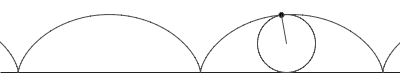
\includegraphics[width=0.6\textwidth]{season3/304/images/cycloid.png} 
	\end{figure}

\fbox{\begin{minipage}{43em}
\begin{center} \large \dotuline{Tangent}  \\ \end{center}
Brachistochrone Problem. An upside down cycloid is the solution to the famous \bref{Brachistochrone problem}{https://en.wikipedia.org/wiki/Brachistochrone_curve} (curve of fastest descent) between two points; that is, the curve between two points that is covered in the least time by a body that starts at the first point with zero speed under the action of gravity and ignoring friction. This problem was solved posed in the \emph{Acta Eruditorum}, the first scientific journal of Germany, in 1696. The problem was solved by 4 famous mathematicians: Isaac Newton, Jakob Bernoulli, Gottfried Leibniz, and Guillaume de l'H\^{o}pital.
\end{minipage}} \vspace{0.2cm}

In few words, it is the curve described by looking at the movement of a point on a circle while we move the circle along a straight line. In the activity below we study the mathematical equations that describe this curve. \\

\fbox{\begin{minipage}{43em}
\begin{center} \large \dotuline{Activity 2}  \\ \end{center}
\begin{enumerate}[i.]
\item Consider the figure to the right and argue that the distance between $O$ and $A$ is $ra$.
\item Using the result from above, what is the value of $x$ in terms of $a$ and $r$? [Hint: Use trigonometric functions.]
\item What is the value of $y$? [Hint: Use trigonometry again.]
\item Compute the length of the segment of the curtate cycloid that has been drawn in the picture below.
	\begin{figure}[H]
	   \centering
	   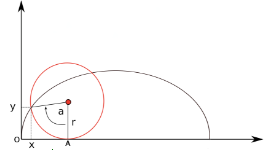
\includegraphics[width=0.5\textwidth]{season3/304/images/cycloidsetup.png} 
	\end{figure}
\end{enumerate}
\end{minipage}} \vspace{0.2cm}


%%%%%%%%%%
\temph{Branching and Bounding}
%%%%%%%%%%

Charlie uses this \emph{combinatorial optimization} technique to predict the next meeting between Carter and the Chinese.

\noindent\textbf{\large Combinatorial Optimization Problems}

Before describing this technique, we say something about combinatorial optimization problems. One such problem is the following ``Find the pair of positive integers whose sum is 100, and whose product is as big as possible.'' In this case we are trying to maximize the two-variable function \emph{product of two integers}, which is defined by $f(x,y) = xy$. $f$ is called the \emph{objective function}. Notice that the set $S$ of non-negative integers in which we are interested is described by the equation $x + y = 100$. The set $S$ is called the set of feasible solutions. In other words, a combinatorial optimization problem consists of these ingredients:
	\begin{itemize}
	\item The problem is to minimize a function $f(x)$ of variables $x_1$, $x_2$, $\ldots$, $x_n$ over a region of feasible solutions $S$. That is, we are interested in finding 
	\[
	\max_{x \in S} f(x) \text{ or } \min_{x \in S} f(x), \text{ respectively}
	\]
	\item The set $S$ is usually determined by general conditions on the variables, such as them taking values on the non-negative integers.
	\end{itemize}

In out example, we can just go ahead and try every single element in S to find which pair maximizes the objective function $f$. Of course there are many techniques to find the optimal solution, depending on the particular problem. Branching and bounding algorithms constitute one such technique. \\


\noindent\textbf{\large B\&B Algorithms}

There exists a combinatorial optimization technique called branching and bounding (hereinafter called B\&B) which basically consists of searching for the best solution among all possible solutions to a problem by dividing the set of solutions and using bounds for the function to be optimized. Since there is some enumeration of solutions involved in the process, this technique can perform very badly in the worst case; however, the integration of B\&B algorithms with other optimization techniques and has proved useful for a wide variety of problems. \\

Here is a description of the three main components involved in B\&B algorithms for minimization problems (with the case for maximization problems dealt with similarly):
	\begin{enumerate}[1.]
	\item A \emph{bounding function} (upper or lower, depending on the case) $g(x)$ for our objective function $f$ that will allow us to discard some subsets of $S$.
	\item A \emph{branching rule} that tells us how to divide a subset of $S$ in case we are not able to discard such a subset as not having the optimal solution which we are looking.
	\item A \emph{strategy} for selecting the subset to be investigated in the current iteration. 
	\end{enumerate}


\fbox{\begin{minipage}{43em}
\begin{center} \large \dotuline{Tangent}  \\ \end{center}
B\&B algorithms are an example of \bref{divide and conquer algorithms}{https://en.wikipedia.org/wiki/Divide_and_conquer_algorithm}. The idea is to break the problem down to smaller problems that are easy to solve. This technique has proved useful in solving instances of the \bref{traveling salesmen problem}{https://en.wikipedia.org/wiki/Travelling_salesman_problem} with 40 to 60 cities and the \bref{graph partitioning problem}{https://en.wikipedia.org/wiki/Graph_partition}.
\end{minipage}} \vspace{0.2cm}


We describe the technique with the following example: \\

\noindent\textbf{Example:} Maximize the function $z= 21x_1 + 11x_2$ given the constraints $7x_1 + 4x_2 \leq 13$, with $x_1$ and $x_2$ non-negative integers. \\

\noindent\textbf{Solution:} The set $S$ is described by the inequalities $7x_1 + 4x_2 \leq 13$, $x_1 \geq 0$, $x_2 \geq 0$. Since we cannot discard $S$, we subdivide it into smaller pieces, thus making the original problem smaller. For instance, let us focus on the subset of $S$ where $x_2 = 0$. Then $z$ attains its maximum when $x_1 = 13/7 \approx 1.857$. \\

This first step was used as our branching rule, and now we focus on two subsets of $S$, $S_1$ and $S_2$ as shown in the picture below. We easily see that there are no feasible solutions on $S_2$, and that the solution on $S_1$ is $z = 37.5$, which is attained with $x_1 = 1$, and $x_2 = 1.5$; this value of $x_2$ is used as our new branching rule. We now consider the problem in two new subsets, $S_{11} = \{\text{solutions with } 0 \leq x_1 \leq 1 \text{ and } 0\leq x_2 \leq 1\}$ and $S_{12} = \{\text{solutions with }0 \leq x_1 \leq 1 \text{ and } x_2 \geq 2\}$. Solving the original problem (maximizing $z$) for $S_{12}$ yields $z = 37$, which is attained by $x_1 = 0.71$ and $x_2 = 2$, so we branch at $x_2$ once again and consider the sets $\{x_1 = 1, x_2 \geq 2\}$ and $\{x_1 = 0 \text{ and } x_2 \geq 2\}$. Finally, the solution must be in $S_{11}$, and solving the original problem on this set yields $z = 32$, which is attained by $x_1 = x_2 = 1$. Continuing in this matter, we obtain the answer $z = 33$, which is attained when $x_1 = 0$ and $x_2 = 3$. This answer is in the set $S_{1211}$.
	\begin{figure}[H]
	   \centering
	   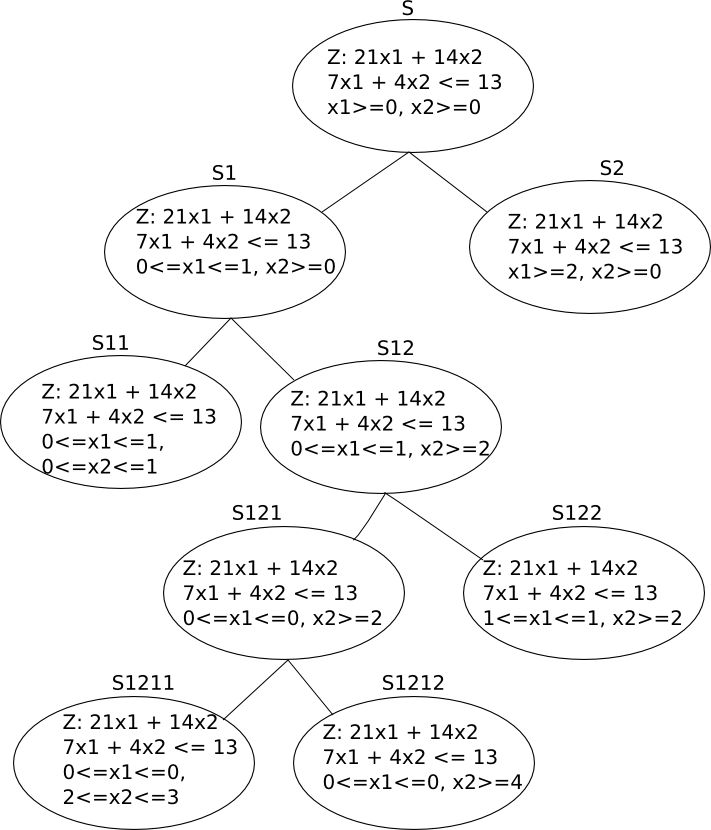
\includegraphics[width=0.5\textwidth]{season3/304/images/bb.png} 
	\end{figure}
The picture above depicts the process used to solve our problem. We considered 9 subsets of $S$; that is, the number of vertices in the graph depicted above is 9. \\


\fbox{\begin{minipage}{43em}
\begin{center} \large \dotuline{Activity 3}  \\ \end{center}
\begin{enumerate}[a.]
\item Using the procedure just explained, to maximize $2x + 3y$, given that $10x + 3y \leq 24$, for non-negative integers $x$ and $y$.
\item Maximize $-x + y$, given that $12x + 11y \leq 63$, $-22x + 4y \leq -33$, for non-negative integers $x$ and $y$.
\item[c*.] Let $n$ be a positive odd integer. Consider the following optimization problem: Maximize $-x_0$ subject to $x_0+2(x_1+ \cdots + x_n) = n$, $0 \leq x_j \leq 1$ for $j = 0, 1,\ldots, n$, where all the variables are integers. Show that the number of subsets that need to be consider (number of vertices in the graph) is at least $2^{(n-1)/2}$.
\end{enumerate}
\end{minipage}} \vspace{0.2cm}

















